\documentclass{article}

\usepackage[margin=1in]{geometry}     %for 1inch margins that play nice with fancyhdr
\usepackage{amsmath,amssymb}          % math and junk
\usepackage{fancyhdr}                 % for a nice running header and footer
\usepackage{lastpage}                 % for nice "X of Y" footer
\usepackage[per-mode=symbol,alsoload=binary,detect-all=true]{siunitx}
                                      % for nice units and junk!
\usepackage{gnuplot-lua-tikz}         % enable tikz plots made from gnuplot
\usepackage{float}                    % [H] option for floats
\usepackage[american]{circuitikz}     % for teh circuit diagrams
\usepackage[hidelinks]{hyperref}                 % get those sweet, sweet, links
\usepackage{framed}                   % for framed titlepage
\usepackage{subfig}

\usetikzlibrary{shapes,arrows}

% unused, but common for other experiments
%\usepackage{rotating}                 % for sideways stuff!
%\usepackage{cancel}                   % for `canceling out' parts of equations. fancy!
\usepackage{mdwlist}                  % itemize* and friends
%\usepackage{verbatim}                 % for \verbatiminput command and comment environment
%\usepackage[colorinlistoftodos]{todonotes}                % todo's, if used/needed
%\usepackage{multirow}                 % for multi-row spans in tabular environment


% values!
\newcommand{\docAuthor}{Sean Barag}
\newcommand{\docCoAuthor}{None}
\newcommand{\ta}{Yang Gao}
\newcommand{\docTitle}{Building the DAC Circuit}
\newcommand{\courseName}{ECE-L304}
\newcommand{\labNum}{Step 3}
\newcommand{\labSec}{064}
\newcommand{\dueDate}{10 January 2012}
\newcommand{\perfDate}{1 February 2012}

% paths
\graphicspath{{$HOME/texmf/graphics/}}


% meta-data
\pdfinfo{
	/Title    (\labNum: \docTitle)
	/Author   (\docAuthor)
	/Keywords (\docTitle, \labNum)
}

% for fancy header
\pagestyle{fancy}
\lhead{\courseName\ $|$ \labSec}
\chead{\labNum: \docTitle}
\rhead{\docAuthor}
\cfoot{\thepage\ of \pageref{LastPage}}

% title info
\title{\courseName\ \labNum: \\ \docTitle}
\author{\docAuthor}
\date{}

% shortcuts, cause I'm lazy
\newcommand{\bs}[1]{\boldsymbol{#1}}
\newcommand{\tbf}[1]{\textbf{#1}}
\newcommand{\ttt}[1]{\texttt{#1}}

\begin{document}
% Cover page written by Bryndon Blackburn
% Originally written by Bryndon Blalckburn
\begin{titlepage}
	\begin{center}
		\includegraphics[scale = 0.50]{DrexelLogo.pdf}
	\end{center}

	\large
	\begin{framed}
		\begin{center}
			Electrical and Computer Engineering Dept. \\
			Electrical Engineering Laboratory IV, ECE-L304 \\
		\end{center}
	\end{framed} \vspace{50pt}

	\begin{description}
		\item[Title:]\labNum: \docTitle
		\item[Author:] \docAuthor
		\item[Partner:] \docCoAuthor
		\item[Instructor:] \ta
		\item[Section:] \labSec
		\item[Date Performed:] \perfDate
		\item[Date Due:] \dueDate
		\item[Date Received:]
	\end{description}
\end{titlepage}


% Blank page so two-sided printing leaves the cover page on its own sheet
\thispagestyle{empty}
\newpage
\mbox{}

\maketitle
\setcounter{page}{1} % fixes page numbering issues caused by cover sheet
\tableofcontents % this helps
%\newpage
%\listoffigures   % there's over 9000 figures

\newpage % I want the actual content to be at the top of a new page

\section{Introduction}
The entirety of ECE-L304 is devoted to the design, construction, and debugging
of a digital voice recorder.  By providing students with an opportunity to
complete a project of larger scale than anything they have previously
attempted, the course offers its students valuable skills and experience with a
long-term engineering project.

As the system uses digital storage in the form of a RAM chip, it is necessary
to convert all input audio from its native analog form to a digital
representation.  Similarly, the stored digital representation must be converted
back to an analog signal so that it can be correctly rendered by a speaker.
These conversions are performed by an analog to digital converter (ADC) and a
digital to analog converter (DAC), resepectively.
%
In order to ease the design process, students first complete a simple ADC and
DAC simulation.  This helps to remind students of the operating properties and
behaviors of the two converters, as well as providing a schematic similar to
the one required in the final design.

%\section{Circuit}

\begin{center}
\begin{tikzpicture}
	\draw[fill=red] (0,0) rectangle node {\LARGE CIRCUIT} (8,6);
\end{tikzpicture}
\end{center}

\begin{table}[H]
\centering
	\section{Elements}

After consulting the datasheet for the DAC0808 integrated circuit, it was
determined that three~\SI{5}{\kilo\ohm} resistors were required for the proper
operation of the chip.  The measured values are shown in
Table~\ref{t:elements}, along with the elements used in the construction of the
ADC in step 2 (which utilized the ADC0804 IC).
%
\begin{table}[H]
\centering
	\section{Elements}

After consulting the datasheet for the DAC0808 integrated circuit, it was
determined that three~\SI{5}{\kilo\ohm} resistors were required for the proper
operation of the chip.  The measured values are shown in
Table~\ref{t:elements}, along with the elements used in the construction of the
ADC in step 2 (which utilized the ADC0804 IC).
%
\begin{table}[H]
\centering
	\input{tbl/elements.tex}
	\parbox{.8\textwidth}{
	\caption[List of used elements]{Required, nominal, and measured element
	values used in the ADC and DAC circuits.}
	\label{t:elements}}
\end{table}
%
With errors for the DAC resistors all falling under~\SI{1}{\percent}, the
elements are all appropriately accurate for this application.

	\parbox{.8\textwidth}{
	\caption[List of used elements]{Required, nominal, and measured element
	values used in the ADC and DAC circuits.}
	\label{t:elements}}
\end{table}
%
With errors for the DAC resistors all falling under~\SI{1}{\percent}, the
elements are all appropriately accurate for this application.

	\parbox{.8\textwidth}{
	\caption[List of used elements]{Required, nominal, and measured element
	values used in the ADC and DAC circuits.}
	\label{t:elements}}
\end{table}

\section{Elements}

After consulting the datasheet for the DAC0808 integrated circuit, it was
determined that three~\SI{5}{\kilo\ohm} resistors were required for the proper
operation of the chip.  The measured values are shown in
Table~\ref{t:elements}, along with the elements used in the construction of the
ADC in step 2 (which utilized the ADC0804 IC).
%
\begin{table}[H]
\centering
	\section{Elements}

After consulting the datasheet for the DAC0808 integrated circuit, it was
determined that three~\SI{5}{\kilo\ohm} resistors were required for the proper
operation of the chip.  The measured values are shown in
Table~\ref{t:elements}, along with the elements used in the construction of the
ADC in step 2 (which utilized the ADC0804 IC).
%
\begin{table}[H]
\centering
	\section{Elements}

After consulting the datasheet for the DAC0808 integrated circuit, it was
determined that three~\SI{5}{\kilo\ohm} resistors were required for the proper
operation of the chip.  The measured values are shown in
Table~\ref{t:elements}, along with the elements used in the construction of the
ADC in step 2 (which utilized the ADC0804 IC).
%
\begin{table}[H]
\centering
	\input{tbl/elements.tex}
	\parbox{.8\textwidth}{
	\caption[List of used elements]{Required, nominal, and measured element
	values used in the ADC and DAC circuits.}
	\label{t:elements}}
\end{table}
%
With errors for the DAC resistors all falling under~\SI{1}{\percent}, the
elements are all appropriately accurate for this application.

	\parbox{.8\textwidth}{
	\caption[List of used elements]{Required, nominal, and measured element
	values used in the ADC and DAC circuits.}
	\label{t:elements}}
\end{table}
%
With errors for the DAC resistors all falling under~\SI{1}{\percent}, the
elements are all appropriately accurate for this application.

	\parbox{.8\textwidth}{
	\caption[List of used elements]{Required, nominal, and measured element
	values used in the ADC and DAC circuits.}
	\label{t:elements}}
\end{table}
%
With errors for the DAC resistors all falling under~\SI{1}{\percent}, the
elements are all appropriately accurate for this application.

\section{Results}

For the initial~\SI{10}{\hertz} ramp function~(from zero to five volts), the
length of time devoted to each output voltage segment was measured with an
oscilloscope, as shown in Figure~\ref{f:time_step}.
%
\begin{figure}[H]
\centering
	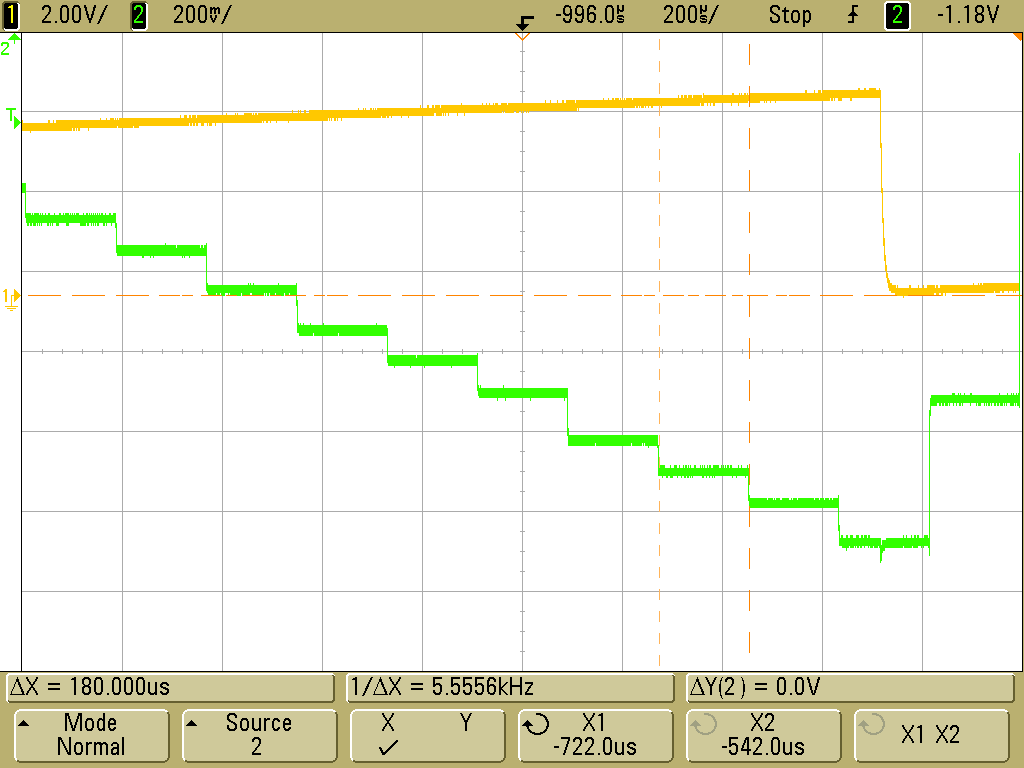
\includegraphics[width=.8\textwidth]{img/shot/ramp_timestep.png}
	\parbox{.8\textwidth}{
	\caption[Segment time]{Oscilloscope screenshot showing the width in time of
	one segment of the DAC output.}
	\label{f:time_step}}
\end{figure}
%
The oscilloscope measured the time step to be~\SI{180}{\micro\second}.  During
this span of time,
%
\begin{equation*}
	\SI{180}{\micro\second} \cdot \SI{379}{\kilo\hertz} = \SI{68.22}{cycles}
\end{equation*}
%
of the internal ADC clock pass (note that the clock frequency
of~\SI{379}{\kilo\hertz} was measured in step two).  This logically makes
sense, as it was observed in step two that each ADC measurement requires
roughly~70 clock cycles, and the ADC output is being directly fed into the
DAC's input in this step.

A similar test was performed with a sinusoidal signal of varying input
frequencies.  For very low frequency inputs, the output waveform closely mimicked
the input, as shown in Figure~\ref{f:100hz} for a~\SI{100}{\hertz} sine wave.
%
\begin{figure}[H]
\centering
	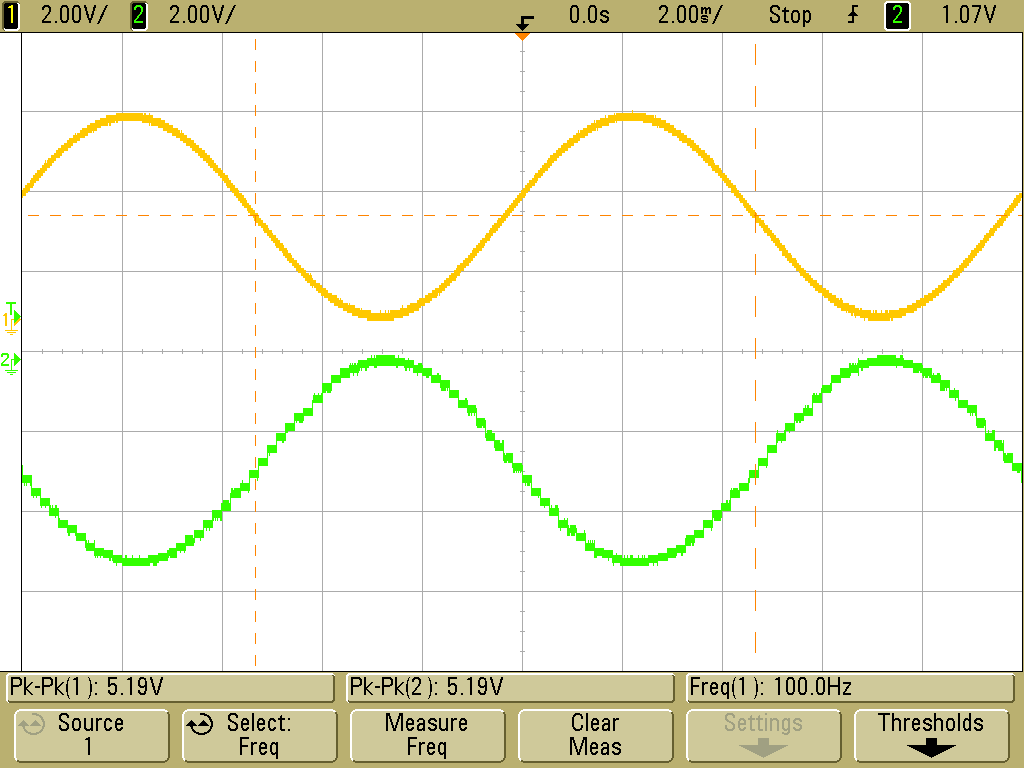
\includegraphics[width=.8\textwidth]{img/shot/sine_100hz.png}
	\parbox{.8\textwidth}{
	\caption[Sinusoidal input --- Low frequency]{Captured input~(upper) and output~(lower) of
	the ADC-DAC circuit.  Note the similarity between the two signals.}
	\label{f:100hz}}
\end{figure}

For high-frequency sinusoidal inputs, the system failed to accurately recreate
the input signal.  For the case of the built circuit, this failure occurred
at~\SI{3000}{\hertz}, shown in Figure~\ref{f:3000hz}.
%
\begin{figure}[H]
\centering
	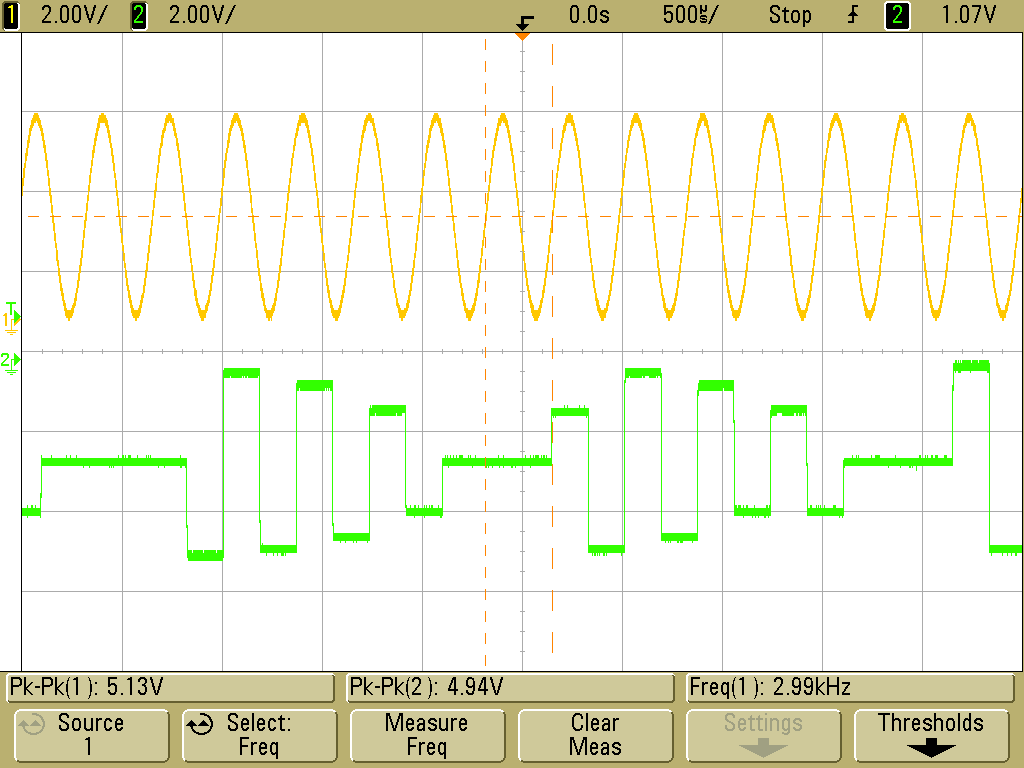
\includegraphics[width=.8\textwidth]{img/shot/sine_3000hz.png}
	\parbox{.8\textwidth}{
	\caption[Sinusoidal input --- Failure]{Failed recreation of the input
	signal by the combined ADC-DAC system.  This oscilloscope screenshot was
	captured for a sinusoidal input of~\SI{3}{\kilo\hertz}.}
	\label{f:3000hz}}
\end{figure}
%
A sinusoid of~\SI{3000}{\hertz} has a period of
just~$0.33\overline{3}\si{\micro\second}$ --- a period that is an order of
magnitude below the~\SI{2.639}{\micro\second} period of the internal ADC clock.
A signal with such a small period is impossible to represent with such a slow
clock frequency, and results in the aliasing shown in Figure~\ref{f:3000hz}.
As the internal ADC clock is set by the values of the resistor and capacitor
for the ADC, adjusting the clock frequency is a non-trivial task that changes
the overall performance of the system.


\newpage
\appendix
\section{License}
\section{License}

Copyright \copyright\ 2011, Sean Barag.  All rights reserved.

Redistribution and use in source and binary forms, with or without
modification, are permitted provided that the following conditions are met:
\begin{itemize}
\item Redistributions of source code must retain the above copyright notice, this
  list of conditions and the following disclaimer.
\item Redistributions in binary form must reproduce the above copyright notice, this
  list of conditions and the following disclaimer in the documentation and/or
  other materials provided with the distribution.
\item Neither the name of the owner nor the names of its contributors may be
  used to endorse or promote products derived from this software without specific
  prior written permission.
\end{itemize}

THIS SOFTWARE IS PROVIDED BY THE COPYRIGHT HOLDERS AND CONTRIBUTORS ``AS IS'' AND
ANY EXPRESS OR IMPLIED WARRANTIES, INCLUDING, BUT NOT LIMITED TO, THE IMPLIED
WARRANTIES OF MERCHANTABILITY AND FITNESS FOR A PARTICULAR PURPOSE ARE
DISCLAIMED. IN NO EVENT SHALL THE COPYRIGHT HOLDER OR CONTRIBUTORS BE LIABLE
FOR ANY DIRECT, INDIRECT, INCIDENTAL, SPECIAL, EXEMPLARY, OR CONSEQUENTIAL
DAMAGES (INCLUDING, BUT NOT LIMITED TO, PROCUREMENT OF SUBSTITUTE GOODS OR
SERVICES; LOSS OF USE, DATA, OR PROFITS; OR BUSINESS INTERRUPTION) HOWEVER
CAUSED AND ON ANY THEORY OF LIABILITY, WHETHER IN CONTRACT, STRICT LIABILITY,
OR TORT (INCLUDING NEGLIGENCE OR OTHERWISE) ARISING IN ANY WAY OUT OF THE USE
OF THIS SOFTWARE, EVEN IF ADVISED OF THE POSSIBILITY OF SUCH DAMAGE.\\

Source code for this document is available at \texttt{http://github.com/sjbarag/}.


\end{document}
